\chapter{Design}\label{chap:3}


This chapter undergoes the design steps that are taken in each stage of the research. Initially this research is started as\textbf{ Compile time server architectures for Ballerina}. After analyzing the results of initial set of experiments, focus area is narrowed down to finding optimal thread pool size for different programming features. A machine learning approach is used to predict the thread pool size for given set of programming features. Research questions remain unchanged from the beginning since thread pools are crucial part in web server architectures and it is a tuning parameter for further improving the performance of server architecture. Literature review indicates that performance of single web server architecture differ according to type of operations it executes. Type of the operations can be extracted by analysing the source code.  In simple terms different web server architecture perform differently for different types of programs. Then based on the results further improvements and fine-tuning to the architecture are carried out in order to identify what parameters are required to change for maximizing the performance for each type of program. 

Formal research methodology is based on Design science research approach \cite{design_science}. Design science research approach requires the creation of an innovative, purposeful artifact for a special problem domain. The artifact must be evaluated in order to ensure its utility for the specified problem. In order to form a novel research contribution, the artifact must either solve a problem that has not yet been solved, or provide a more effective solution. Both the construction and evaluation of the artifact must be done rigorously, and the results of the research presented effectively both to technology-oriented and management-oriented audiences.

This research tries to provide more effective solutions to a current problem and creates innovative solutions by introducing techniques to predict optimal thread pool size based on program features.

Design of the research is devised in to for stage. First off existing Ballerina server architecture is carefully analyses and designed how new architectures can be derived from it. Then new architectures are implemented by modifying the source code. Secondly, identified parameters from fist phase is tuned in order to maximize the performance in server architectures. In this phase size of the thread pool is tuned. Thirdly, differentiate the IO intensive features in program and machine learning model is designed to predict size of the thread pool. Finally, \acrshort{AST} is parsed for extracting the identified features to fed into the model that designed.

This research is consist of following areas. Below sections spans the design steps considered answering the research questions mentioned in section .

Before dive into the design steps, it is important to specify internal architecture of Ballerina run time. Next section briefly explain the internals of the Ballerina.

\section{Ballerina}\label{Sec_Ballerina}

This section provides overview of current Ballerina architecture and explanation on how this research expects to use network awareness features in Ballerina language.  

In Ballerina connector calls that basically perform IO operations are explicitly presented in the source code as “ - $>$“. \acrfull{AST} parser extract this information from the source to identify whether this call is a connector call and type of the connector call (HTTP, Database etc.).

Following is one example how the database calls are represented in ballerina code, note the -$>$ symbol.\\

\textit{stream$<$record{}, error$>$ resultStream = mysqlClient4 - $>$ query(<@untainted>query);}\\

Algorithm used for this operation is presented in section \ref{phase_iv}

\subsection{Ballerina internal architecture}

This section explains the main components of Ballerina run time.

\subsubsection{Netty Layer}

This layer is implemented using a library called Netty \cite{netty}. Primary task of the Netty layer is to listen for Http client connections and manage the session. It has its own thread pools to handle those connections. In original ballerina architecture this layer simply handed over the incoming connection to the ballerina scheduler. Then the scheduler invokes relevant tasks for the client and returns the results to Netty layer again for submitting back to the client. Inside the Netty layer three is two types of threads.(1) \textbf{Boss threads} — Each bonded port has own boss thread. For example, if server listen on ports 80 and 443, then there are two boss threads. Main function of these threads are accepting the client requests. (2) \textbf{Worker threads} — Boss thread passes the accepted request to the worker thread. Worker thread then carry out the execution of task. In Ballerina, these worker threads pass the request to Ballerina scheduler.

\subsubsection{Scheduler}

Ballerina scheduler is the main component for every program/operation which executes. The Ballerina scheduler executes the client request using its own thread pool. The default thread pool size is two times the available processor count of the operating system. All the tasks which need to executed are held in a queue. Then threads in the pool access the queue and execute the task. This is where major turnings are happened at final stage of the research. 

\subsubsection{Resource function}

In ballerina each API endpoint can be implemented as a resource function. That function includes all the implementation required to fulfill the task that client is requested. More details about resource function is stated in Chapter 4. In this research each resource functions are considered as programs.


Figure \ref{bal_internal} shows high level view of Ballerina architecture.

\begin{figure}[htbp]
	\begin{center}
		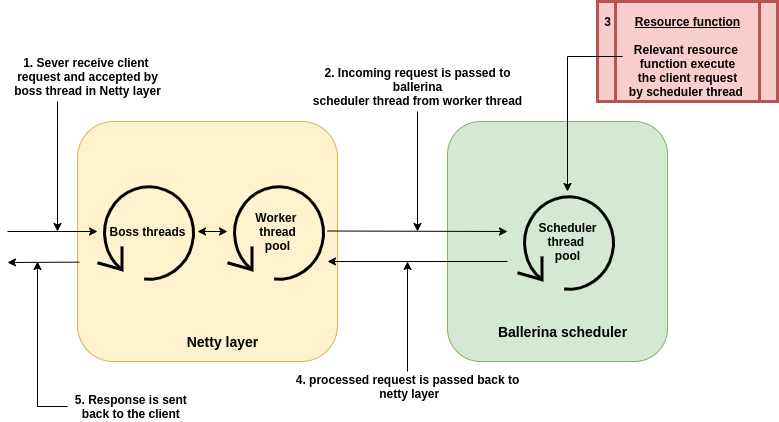
\includegraphics[scale=0.5]{figures/bal-internal.png}
	\end{center}
	\caption{Ballerina's internal architecture}
	\label{bal_internal}
\end{figure}

\section{Design steps}

The initial idea is coupled with bound type of the program (CPU bound and IO bound). Objectives were, (1) for a given Ballerina program identify its bound type, then (2) switch the server architecture which best suits the bound type. To determine the best  server architecture, experiments are conducted. Following steps are taken to conduct the experiments. Below process is iterative.

\begin{itemize}
	\item Implement server architectures
	\item Use existing benchmark programs and implement new programs as necessary which have CPU intensive task and IO intensive tasks.
	\item Examine results.
	\item Debug and fine tune architectures based on results.
\end{itemize} 

\subsection{Testing process}

Each testing program is hosted as HTTP endpoints. Calling that endpoint invokes the relevant program. Jmeter act as a HTTP client. Typical web server able to process concurrent HTTP requests. Jmeter can be configured to model this behavior. Jmeter continuously calls the given endpoint for certain period under given configurations such as concurrency level. Then the following metrics are recorded,

\begin{itemize}
	\item Average latency — client HTTP requests are continuously sent to the web server and measure response time of each request. Then average is calculated.
	\item Standard deviation of latency — Standard deviation of above latency results.
	\item Throughput — Number of success response received per second.
	\item Error rate - Number of erroneous request as percentage of all request sent.
	\item Median, 75th percentile, 99th percentile of latency results.
\end{itemize} 

Then the performance are evaluated using above metrics. As an example when average latency is low and throughput is high for given endpoint, that architecture's performance is good relatively others.
  

\begin{figure}[htbp]
	\begin{center}
		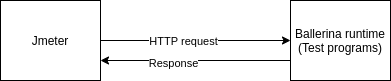
\includegraphics[scale=0.5]{figures/jmeter_bal.png}
	\end{center}
	\caption{Jmeter and Ballerina run time}
	\label{jmeter_testing}
\end{figure}



\subsection{Phase I - Implement and evaluate performance of different server architectures}

In this phase following server architectures are implemented. 

 \begin{itemize}
 	\item Original Ballerina architecture
 	\item Netty OIO
 	\item Removed Ballerina scheduler thread pool
 	\item Changing Ballerina scheduler thread pool size
 \end{itemize} 

The goal of implementing Netty OIO is to have similar architecture of thread per connection model. In this Netty's worker thread pool is configured to spawn new thread per each client request. These thread blocks the execution until task is finished. However, Ballerina scheduler continues the execution in non-blocking fashion.

The expectation of removing Ballerina scheduler is to  inspect the behavior and performance when one thread pool is removed. The Netty layer's worker thread will carry out the execution of client task instead of Ballerina scheduler thread. When there are multiple thread pools, it add some overheard to the system. Expected behavior of removing thread pool is improve the performance. 

Despite that, purpose of having multiple thread pool is to avoid starvation where a task is keeping thread pool busy so that another task is waiting and not getting chance to execute for some time.Therefor that task is starved. instead of having single thread pool for all functions,if other service have their own thread pool, then it is assured of having a certain number of threads at its disposal, hence it's not as sensitive to demands made by other services. The idea is when there are multiple thread pools, while one partition of the application is busy, but other part of the application continue to work normally regardless of rest of the system. This will add more stable characteristics to the system when the load is high.

%The multiple threadpools would require tuning to make sure each pool had enough threads and not too many. With a single threadpool you wouldn't need the tuning and might make better use of all the threads sometimes, but you might not have the predictability of knowing some important task would get the threads it needed to finish in a timely manner.
%

Finally, some variation to number of threads in the Ballerina scheduler is performed. \textbf{Default thread pool size of Ballerina scheduler} is \textbf{$ \boldsymbol{2} \times \boldsymbol{Number\: of\: CPU\: cores}$}. Size of the thread pool is increased by \textbf{$ \boldsymbol{2} \times \boldsymbol{Number\: of\: CPU\: cores}$} and \textbf{$ \boldsymbol{4} \times \boldsymbol{Number\: of\: CPU\: cores}$}. In Ballerina connector calls like database are block the execution thread. Increasing the number of threads can be beneficial in such situation because while other threads are blocking there are more threads to handle other tasks. 

For each architectural changes number of benchmark programs were run which are consist of CPU intensive and IO intensive features.
After conducting experiments with above architectures, following conclusions were made,
 
\begin{itemize}
	\item Netty OIO performance is worse in every situation — thus this architecture was no longer considered
	\item Removing Ballerina scheduler perform well for both IO and CPU intensive programs.
\end{itemize} 

Results are discussed in-depth in Chapter \ref{chap:5}. Based on these results, experiments were conducted with changing size of the thread pool in Ballerina scheduler.

\subsubsection{Test programs}

Following programs were implemented to evaluate the performance of each architectural change,

  \begin{itemize}
  	\item Check whether given number is prime - 3 primes are checked as small (521),medium(7919) and large(1000003)
  	\item Merge sort — 1000 random numbers are sorted
  	\item Read File from disk
  	\item ‘select’ query on mysql database
  \end{itemize} 
Above programs cover the CPU intensive cases and IO intensive cases. 

Sample representation of single experiment is shown in figure \ref{sample_result}. Four metrics (throughput, slandered divination, mean — average latency, 99th percentile  ) are shown in the plot. X-axis represents the concurrent users. Y-axis represents the  relevant metric. 

 \begin{figure}[htbp]
 	\begin{center}
 		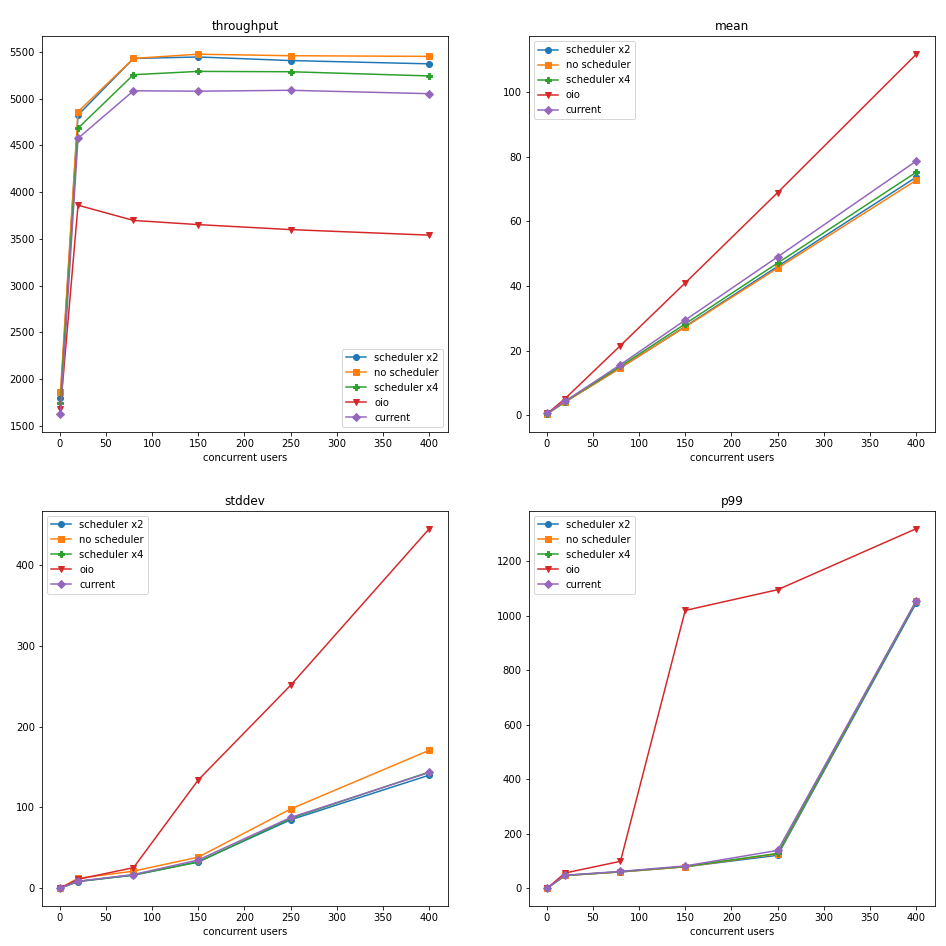
\includegraphics[scale=0.35]{figures/prime_small test results.png}
 	\end{center}
 	\caption{Sample experiment result}
 	\label{sample_result}
 \end{figure}

Then each metric is evaluated against each test program and each architectural changes above mentioned.

\begin{comment}

\begin{table}[]
\begin{center}
\begin{tabular}{|l|l|l|l|l|l|}
\hline
Test case                                                     & \multicolumn{5}{l|}{Server architecture}                                                                                                                                                                                                                                \\ \hline
& \begin{tabular}[c]{@{}l@{}}Ballerina \\ original\end{tabular} & \begin{tabular}[c]{@{}l@{}}No \\ scheduler\end{tabular} & Netty OIO & \begin{tabular}[c]{@{}l@{}}Thread pool\\  size x 2\end{tabular} & \begin{tabular}[c]{@{}l@{}}Thread pool\\  size x 4\end{tabular} \\ \hline
\begin{tabular}[c]{@{}l@{}}Prime check \\ small\end{tabular}  &                                                               &                                                         &           &                                                                 &                                                                 \\ \hline
\begin{tabular}[c]{@{}l@{}}Prime check \\ medium\end{tabular} &                                                               &                                                         &           &                                                                 &                                                                 \\ \hline
\begin{tabular}[c]{@{}l@{}}Prime check \\ large\end{tabular}  &                                                               &                                                         &           &                                                                 &                                                                 \\ \hline
\begin{tabular}[c]{@{}l@{}}Database \\ call (IO)\end{tabular} &                                                               &                                                         &           &                                                                 &                                                                 \\ \hline
Merger sort                                                   &                                                               &                                                         &           &                                                                 &                                                                 \\ \hline
File read                                                     &                                                               &                                                         &           &                                                                 &                                                                 \\ \hline
\end{tabular}
\end{center}
\caption{Architecture comparison metric}
\label{tab:result_metric}
\end{table}

\end{comment}


Architectural changes to existing Ballerina run time involved extensive debugging because bugs in the implementation may incur wrong results. Therefore, this phase is conducted in iterative manner to verify the results.
At end of this stage no architecture was performed well for IO use cases rather than CPU intensive cases and vice versa. Although changing thread pool size in Ballerina scheduler started to show some significance result. Increasing thread pool size was affected differently in IO use cases. Then the phase 2 is designed to analyze the variation of thread pool comprehensively.

\subsection{Phase II - Tuning thread pool size}

Thread pool tuning can be approached is two ways, \textbf{(1) White box system} — This requires complex mathematical modeling with queuing theories \cite{math_aproach_thread_pool_tuning}. Also, assumption made at the beginning make difficult to apply those modeling techniques for practical scenarios. \textbf{(2) Black box system} — In this approach thread pool system is considered as a black box where in depth analysis of the thread pool system not performed. Experiments are performed heuristically by changing parameters such as size of the thread pool. Figure \ref{black_box_boundary} shows boundary of the black box.

 
\begin{figure}[htbp]
	\begin{center}
		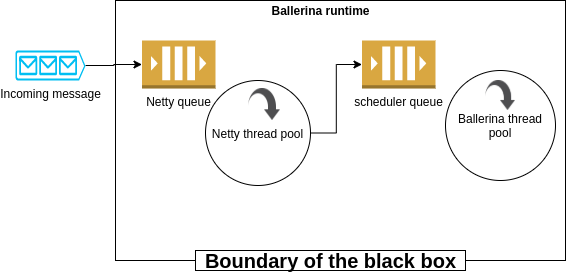
\includegraphics[scale=0.5]{figures/black_box_boundary.png}
	\end{center}
	\caption{Boundary of the black box}
	\label{black_box_boundary}
\end{figure}


This phase is proceeded by considering the system as black box. This model allows executing different programs under different size of thread pool. Following first phase of experiments, it is identified that changing thread pool size is affected differently for programs that consist of IO features. In the previous phase, experiment are conducted under different concurrency level, but in this phase fixed concurrency level is selected. Concurrency level was selected where a number near the point in throughput curve which curve is starting to get flatten.

New set of programs are implemented referring multiple sources \cite{Ballerina_Performance,Ballerina_Website} in order to support programs that have rich IO calls variations. Addition to the database calls in previous phase programs which have remote HTTP calls, GRPC calls and loops that contain these features are implemented. Subsection \ref{sub:phase3} provide more information. CPU intensive programs are no longer considered since it is difficult to extract CPU intensive operations directly by parsing AST. More IO oriented approach is used where AST parser able to extract this information directly from the source code.  
	
\subsubsection{Experimental design} 

As a primary metric of evaluation average latency is used. Then each program is run under different thread pool sizes. Afterward metrics are recorded. Table \ref{tab:pool_size_latency} shows summery of the results. Empty cells represent the average latency. Minimum latency value provide the optimal thread pool size for given program. Instead of declaring thread pool size as multiplier of number of CPU, explicit numbering is used for in-depth analysis of every thread pool size from 1 to 22. This range is selected because latency is always getting higher when increasing the number further.  

\begin{table}[]
	\caption{Program vs. Thread pool size - Latency results}
	\begin{center}
	\begin{tabular}{|l|l|l|l|l|l|l|}
		\hline
		Program    & \multicolumn{6}{l|}{Pool size}        \\ \hline
		& 1            & 2 & 3 & ... & 19 & ... \\ \hline
		Program 1  & Ave. latency    & ...  & ...  & ...  &... &     \\ \hline
		Program 2  &      ...        & ...  & ...  & ...  &... &     \\ \hline
		Program 3  &      ...        & ...  & ...  & ...  &... &     \\ \hline
		...        &      ...        & ...  & ...  & ...  &... &     \\ \hline
		Program 50 &      ...        & ...  & ...  & ...  &... &     \\ \hline
		...        &      ...        & ...  & ...  & ...  &... &     \\ \hline
	\end{tabular}
	\end{center}
	\label{tab:pool_size_latency}
\end{table}

\subsection{Phase III - Building machine learning model to predict optimal thread pool size for given program}\label{sub:phase3}

At first two models are considered addition to predicting optimal thread pool. One model directly predict the latency with given program features and given thread pool size. This model can be expressed as following function. 

$$ Latency \:(ms) = f(\:Program\:features,\:Threadpool\:size\:)$$

Weakness of this model is it heavily depend on nature of IO call. As an example latency is dependent on where the database is hosted if the given program has database call. Also, latency is affected by the network connection also. Then the generalization of result is very difficult.

The next model predict optimal thread pool size for the given program. That model can be expressed as follows. That is the hypothesis that try to resolve using machine learning model. 

$$ Optimal\:thread\:pool\:size = f(\:Program\:features)$$

In order to build this model it is required find the minimum thread pool value from the result obtained by Design phase II. This step can be depicted as in figure \ref{optimal_pool_size}

\begin{figure}[htbp]
	\begin{center}
		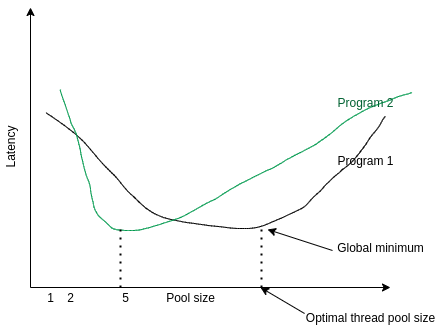
\includegraphics[scale=0.5]{figures/optimal_pool_size.png}
	\end{center}
	\caption{Obtaining optimal thread pool size}
	\label{optimal_pool_size}
\end{figure}

After some feature engineering steps, Features in table \ref{tab:programming-features}  are selected to train the machine learning model. Hyper parameters of each machine learning model is tuned for better accuracy. Implementaion of hyper parameter tuning is presented in chapter \ref{chap:4}.

\begin{table}[]
	\caption{Programming features selected for machine learning model}
	\label{tab:programming-features}
	\begin{tabular}{|l|l|}
		\hline
		& Feature                                                      \\ \hline
		F1 & Number of HTTP connector calls                               \\ \hline
		F2 & Number of Database connector calls                           \\ \hline
		F3 & Number of non-blocking gRPC connector calls                  \\ \hline
		F4 & Number of loops containing HTTP connector calls              \\ \hline
		F5 & Number of loops containing Database connector calls          \\ \hline
		F6 & Number of loops containing non-blocking gRPC connector calls \\ \hline
	\end{tabular}
\end{table}

Then a training data set is created where input features are above programming features and output is optimal thread pool size. Table \ref{tab:data_frame} shows the shape of the data frame.


	\begin{table}[]
		\caption{Data frame shape}
		\label{tab:data_frame}
		\begin{center}
		\begin{tabular}{|l|l|l|l|l|l|}
			\hline
			\multirow{2}{*}{Program} & \multicolumn{4}{l|}{Features} & \begin{tabular}[c]{@{}l@{}}Thread pool\\  size\end{tabular} \\ \cline{2-6} 
			& F 1    & F2    & ..    & Fn   &                                                             \\ \hline
			Program 1                &        &       &       &      &                                                             \\ \hline
			...                      &        &       &       &      &                                                             \\ \hline
		\end{tabular}
	\end{center}
		
	\end{table}

Then following machine learning models are selected and evaluated the accuracy of each model.

\begin{itemize}
	
	\item XGBoost
	\item Support Vector Machine
	\item Decision Tree
	\item Random Forest
	
\end{itemize}

For regression models \acrfull{MAPE} and \acrfull{MSE} are evaluated. For classification models F1 score and accuracy are evaluated.

The problem is originally a regression problem because output of the model is a number. As this research provide a proof of concept, the problem is formulated as classification model as well. Mapping the problem into a classification is possible because, in the result of optimal thread pool sizes, clear clusters  can be recognized. Furthermore, distribution of optimal thread pool is not uniform and only has several values.

\subsection{Phase IV - Parsing Ballerina AST to obtain features}\label{phase_iv}

First off, it is better have some idea about what is \acrfull{AST}. It is a tree representation of stricture of the source code.AST does not include all the details such as semicolon, parenthesis etc. AST is used in semantic analysis of a code during compilation process. Traversal of the AST verify the correctness of the program against rules provided for that language. Moreover, information of the code can be extracted by traversing the AST.  Example of an AST is shown in figure \ref{AST_example} for code segment shown in figure \ref{code_for_ast}.

\begin{figure}[htbp]
	\begin{center}
		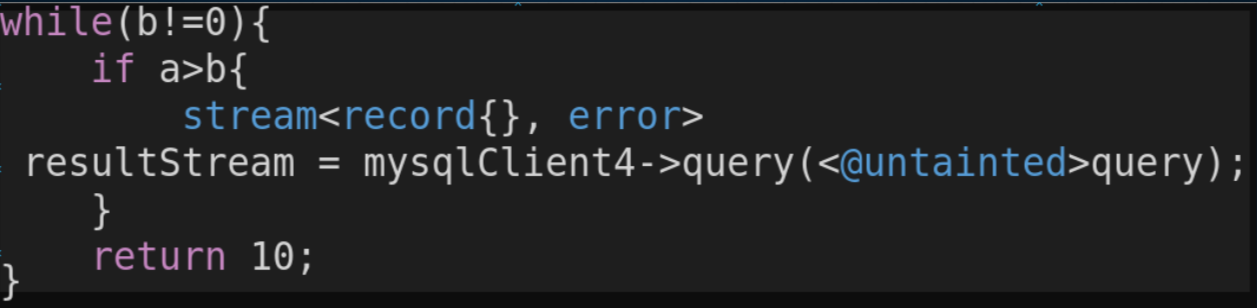
\includegraphics[scale=0.3]{figures/sample_code_for_ast.png}
	\end{center}
	\caption{Ballerina code}
	\label{code_for_ast}
\end{figure}

\begin{figure}[htbp]
	\begin{center}
		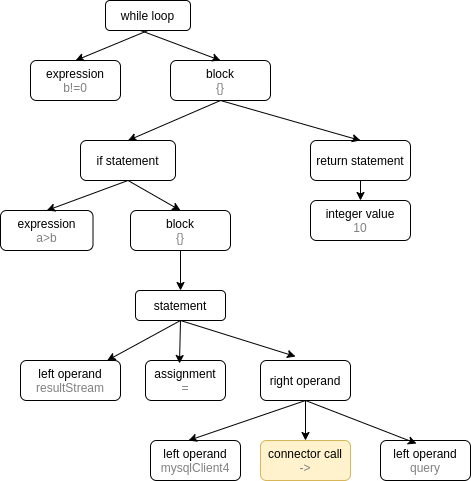
\includegraphics[scale=0.5]{figures/AST example.png}
	\end{center}
	\caption{Example AST}
	\label{AST_example}
\end{figure}

In this phase a module is designed to parse Ballerina source code to feed the features in to machine learning model. Manual feature extraction is erroneous and harder when programs are large. First this module accepts the Ballerina source code and output the array of features which is fed to machine learning model. This is where Ballerina specific features are used that other language are lacks. 
Services are first order functions in the Ballerina language. This able to decide that the given program contain the web service. Then the subsequent parsing are happened inside these service definitions. Also network calls are part of the language. In the other languages they are mostly library calls which is difficult to identify the given line of code contain the network call. In Ballerina this is called as connector call. Recalling section \ref{Sec_Ballerina}, other languages provide network operations as library functions. If we try to extract such features from other languages, we need to know exactly this function call do an IO operation. In Ballerina, it is possible because connector calls can be differentiated naively. Algorithm \ref{alg:ast_parser} is implemented to extract features.

\begin{algorithm}
	\label{alg:ast_parser}
	\SetAlgoLined
	\KwIn{Source code (Ballerina.toml) }
	\KwOut{Feature Array}
	Start parsing\;
	
	\While{End program}{
		
		Traverse node\;{
			\If{Right Arrow Found}{
				
				\If{Left operand is Kind(Database call)}
				{
					\While{Backtrack}{
						
						\If{Loop start found}{
							Update feature array (Database call inside loop + 1)\;
							Stop backtracking and continue parsing\;
						}
						
						Update feature array (Direct Database call + 1)\;
						Continue parsing\;
					}
					
				}
			
				\If{left operand is Kind(Http call)}
				{
					\While{Backtrack}{
						
						\If{Loop start found}{
							Update feature array (HTTP call inside loop + 1)\;
							Stop backtracking and continue parsing\;
						}
						
						Update feature array (Direct HTTP call + 1)\;
						Continue parsing\;
					}
					
				}
			
				\If{left operand is Kind(GRPC-non-blocking call)}
				{
					\While{Backtrack}{
						
						\If{Loop start found}{
							Update feature array (GRPC call inside loop + 1)\;
							Stop backtracking and continue parsing\;
						}
						
						Update feature array (Direct GRPC call + 1)\;
						Continue parsing\;
					}
					
				}
				
			}
		}
		
			
	}
	
	\caption{Extract features using Ballerina AST}
\end{algorithm}

Finally, combing the above design steps, overall design of the research is shown in figure \ref{hl_architecture}.

\section{Limitations}

There are several limitations can be reorganized in  the design. In design phase II, fixed concurrency level is chosen. It is not explored how different concurrency levels are affected to the results. Another limitation is that  hardware variables like number of CPU, memory are not considered when constructing the hypothesis. Finally, when constructing the machine learning model it is only considered IO features. CPU extensive programs cannot be identified by parsing the source code.

